\section{Installazione}
In questa sezione vengono specificati i requisiti necessari per la corretta installazione del sito.
\subsection{Requisiti}
\begin{itemize}
\item Server HTTP Apache;
\item PHP versione 7.0 o superiore;
\item Un database engine compatibile, ad esempio MariaDB.
\end{itemize}

\subsection{Configurazione}
\begin{itemize}
\item Supporto alle istruzioni relative a DirectoryIndex e FallbackResource di Apache;
\item Estensione mysqli di PHP.
\end{itemize}
Non è invece richiesta l'abilitazione del modulo rewrite di Apache.\\
È possibile usare un server HTTP diverso da Apache, ma in tal caso bisogna fare in modo che tutte le richieste puntino al file header.php, in modo da preservare il comportamento del sito.
In caso il sito venga spostato in una directory diversa, bisogna assicurarsi che le istruzioni DirectoryIndex e FallbackResource puntino al file header.php.
\newpage
\subsection{Struttura Directory}
La struttura delle directory del progetto è la seguente:

\begin{figure}[H]
	\begin{center}
		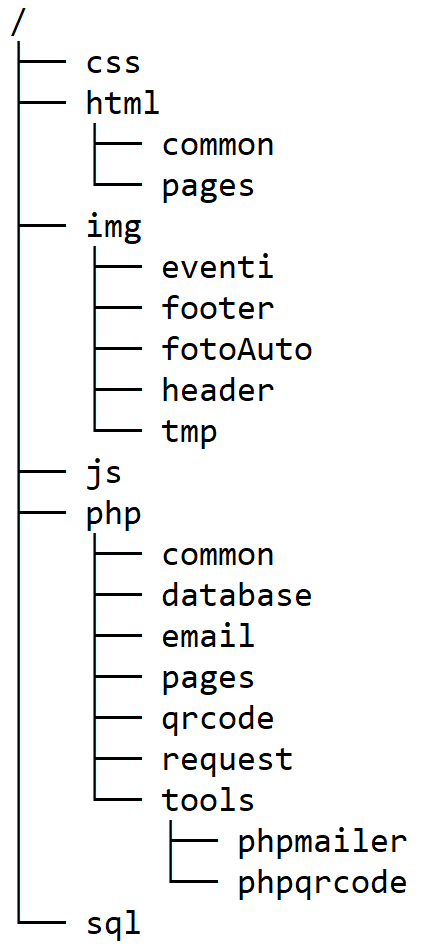
\includegraphics[scale=1.2]{Images/albero.png}
		\caption{Struttura delle directory del progetto}
	\end{center}
\end{figure}

\subsection{Server HTTP Apache}
Per Apache è presente un file .htaccess nella directory / del progetto.
Tale file è molto importante perché il sito mantenga il comportamento corretto lato server.
In caso si usi un server http diverso sarà necessario scrivere le istruzioni necessarie per inoltrare le richieste al file header.php, contenuto nella directory /php/common.